\section{Author Summary} 
\epistasisEnviroAuthorSummary

\section{Introduction}

Epistasis refers to the phenomenon wherein mutations of two genes can
modify each other’s phenotypic outcomes. It can be positive
(alleviating), or negative (aggravating), when a combination of
deleterious mutations shows a fitness value that is higher, or lower,
than expectation, respectively. For example, a mutation that hampers a
pathway's function may allow for other mutations in the same pathway
without a fitness consequence, resulting in positive
epistasis. Conversely, genes or pathways with redundant functions can
give rise to negative epistasis. It is well established that epistasis
is important for the evolution of sex \citep{Kondrashov1982,
Azevedo2006, Otto2007}, speciation \citep{Presgraves2007}, mutational
load \citep{Hansen2001}, ploidy \citep{Musso2008}, genetic
architecture of growth traits \citep{Xu2011}, genetic drift
\citep{Perez-Figueroa2009}, genomic complexity \citep{Sanjuan2008},
and drug resistance \citep{Trindade2009}. As biological systems in
nature have to face multiple genetic
and environmental perturbations, understanding the global landscape
and dynamics of epistasis under these perturbations remains an
important issue in the evolutionary field. In an earlier study, we
addressed genome-wide epistasis dynamics under various genetic
perturbations \citep{Xu2012}. In this study, we will investigate the impact of
environmental perturbations on global epistasis dynamics.

How epistatic interactions among genes change in different
environmental conditions has been intensively studied in various model
organisms, including \textit{E. coli} \citep{Remold2001,
Kishony2003, Cooper2005}, \textit{S. cerevisiae} \citep{Korona1999,
Szafraniec2001, Jasnos2008}, \textit{C. elegans}
\citep{Vassilieva2000, Baer2006} and \textit{D. melanogaster}
\citep{Yang2001, Fry2002, AletheaD.Wang2009}. The results of these
studies, however, are very controversial. While some studies observed
increasing positive epistasis under harsh conditions
\citep{Kishony2003, Jasnos2008, Yang2001}, others have opposite
findings \citep{Cooper2005, Korona1999, Szafraniec2001, Vassilieva2000,
Baer2006, Fry2002, AletheaD.Wang2009, Young2009}. Even within the same
species, different experimental studies might have conflicting
conclusions (e.g. \citealt{Kishony2003, Cooper2005}). One possible
reason for the above controversy could have
originated from the fact that most studies only looked at the
epistasis dynamics based on a small number of genes, where the
properties cannot be generalized to the entire organism.

The main obstacle to exploring global epistatic dynamics under a
variety of environments is the difficulty of applying high-throughput
experimental platforms. To explore epistasis on a genomic scale, a
number of technologies have been developed to systematically map
genetic interaction networks, such as synthetic genetic array (SGA)
\citep{Tong2004, Costanzo2010}, diploid-based synthetic lethality
analysis with microarrays (dSLAM) \citep{Pan2004, Pan2006}, synthetic
dosage-suppression and lethality screen \citep{Measday2002,
Measday2005, Sopko2006} and epistatic miniarray profiles (EMAP)
\citep{Collins2007, Fiedler2009, Kornmann2009}. A key issue for all
these experimental studies is that these epistatic networks have been
constructed only under normal laboratory
conditions. However, cells are constantly bombarded by various
external environmental stresses. Epistasis dynamics under these
perturbations cannot be predicted based on normal laboratory
conditions. Few studies have constructed epistatic networks under
multiple environmental perturbations. A recent study that has only
constructed epistatic networks for a group of genes with specific
functions under one normal and one harsh condition already requires a
large amount of effort \citep{Bandyopadhyay2011}. Consequently,
genome-scale epistasis landscapes under a variety of environmental
perturbations remain largely uncharacterized.

Here we explored this issue by using Flux Balance Analysis (FBA) to
simulate epistasis dynamics among genes under multiple environmental
perturbations. FBA involves optimization of an objective function,
commonly growth maximization in microbes, subject to the reactions and
constraints of a metabolic network, which can provide reliable
predictions \citep{Edwards2001, Shlomi2005, Becker2007, Feist2008,
Smallbone2009a, Orth2010}. Using this platform, a previous study has
investigated synthetic lethal interactions (one type of negative
epistasis) under multiple environmental perturbations and showed the
plasticity of epistatic interactions in the metabolic networks
\citep{Harrison2007}. Here we examined both positive and negative
epistasis using FBA,
and were able to show that at the genome scale epistatic interactions
tend to become more positive in nutrient-limiting conditions relative
to abundant-glucose media. In addition, while a large proportion of
epistatic interactions can be rewired dynamically under varying
environments, there is a core of epistatic interactions that are
stable across all tested environments. We also discovered different
network and evolutionary properties for genes with stable and dynamic
epistatic interactions. Implications of our findings were discussed.

\section{Results}

\subsection{FBA modeling and simulated growth conditions}

We applied the yeast \textit{S. cerevisiae} metabolic reconstruction
iMM904 \citep{Mo2009} to examine the dynamics of epistasis under various
environmental perturbations. The reconstruction has 904 metabolic
genes that are associated with 1,412 metabolic reactions. We conducted
FBA simulations under an abundant-glucose condition and 16
nutrient-limiting conditions with the following environmental
perturbations. In 15 of these perturbations, the carbon source
(abundant glucose) was replaced by one of the following: acetaldehyde,
acetate, adenosine 3',5'-bisphosphate, adenosyl methionine, adenosine,
alanine, allantoin, arginine, ethanol, glutamate, glutamine, glycerol,
low glucose, trehalose, and xanthosine, respectively. These conditions
represent a wide variety of nutrient and energy sources: nucleosides,
amino acids, sugars, alcohols, etc. Additionally, we looked at
abundant glucose under limited phosphorus availability.

To ensure that all these environmental conditions have the same growth
rates in the following analyses, we restricted the carbon source or
phosphorous uptake levels for each of the 16 environmental
perturbations such that only 20\% of the high-glucose growth rate was
attained. This was chosen because it has been shown that metabolism
was directly linked to growth and similar growth rates often induced
similar metabolic pathways \citep{Jakubowska2012}. It is therefore
important to use a fixed growth rate among different conditions to
control for the relationship between growth rates and the overall
metabolic activity so as not to induce a growth-rate specific
effect. The 20\% high-glucose level was chosen because some media
types do not support high growth rates, regardless of the abundance of
the nutrient source. In order to estimate epistasis between genes, we
created a mutation for each gene in each condition that restricted the
flux to be 50\% of the wild-type flux found by geometric FBA for all
reactions associated with the mutant gene \citep{Xu2012}. Epistatic relations
between any two genes were calculated under each condition. We also
tested our core findings allowing maximum growth in each condition
(Table S1) and the general trends in our results remained similar, as
described in the following.

\subsection{More positive differential epistases from rich media to
nutrient-limiting conditions}

To directly address how the sign and magnitude of epistases change
under nutrient-limiting conditions, we calculated differential
epistasis ($\D\epsilon$), which is defined as the epistatic changes from
abundant-glucose media to the nutrient-limiting condition for each
gene pair in each growth condition. A gene pair with positive (or
negative) differential interaction under an environmental perturbation
is defined as these two genes having increasing (or decreasing)
epistasis values from the abundant-glucose media to that
condition. Figure~\ref{fig:eef1}A depicts the distribution of differential
epistases in two growth conditions (ethanol and glycerol) as an
example. Only genes with $\left|\D\epsilon\right| \geq 0.01$ in at least
one of the two conditions are included in this figure. As quantified
in Table S2, there are 6.1\% and 5.5\% of total gene pairs with
$\left|\D\epsilon\right| \geq 0.01$ from abundant-glucose media to ethanol
and glycerol growth conditions, respectively. Among them, a large
number of gene pairs even change their sign of epistasis (Table
S2). Simulations in other conditions show similar effects (Table S2),
indicating that epistatic relationships among genes can be very
dynamic between abundant-glucose media and nutrient-limiting
conditions.

\ifthenelse{\boolean{thesisStyle}}{% 
\captionpage{figure}{%
\eeFBAfigOneCap}
\label{fig:eef1}

\begin{figure}[H]
\centering
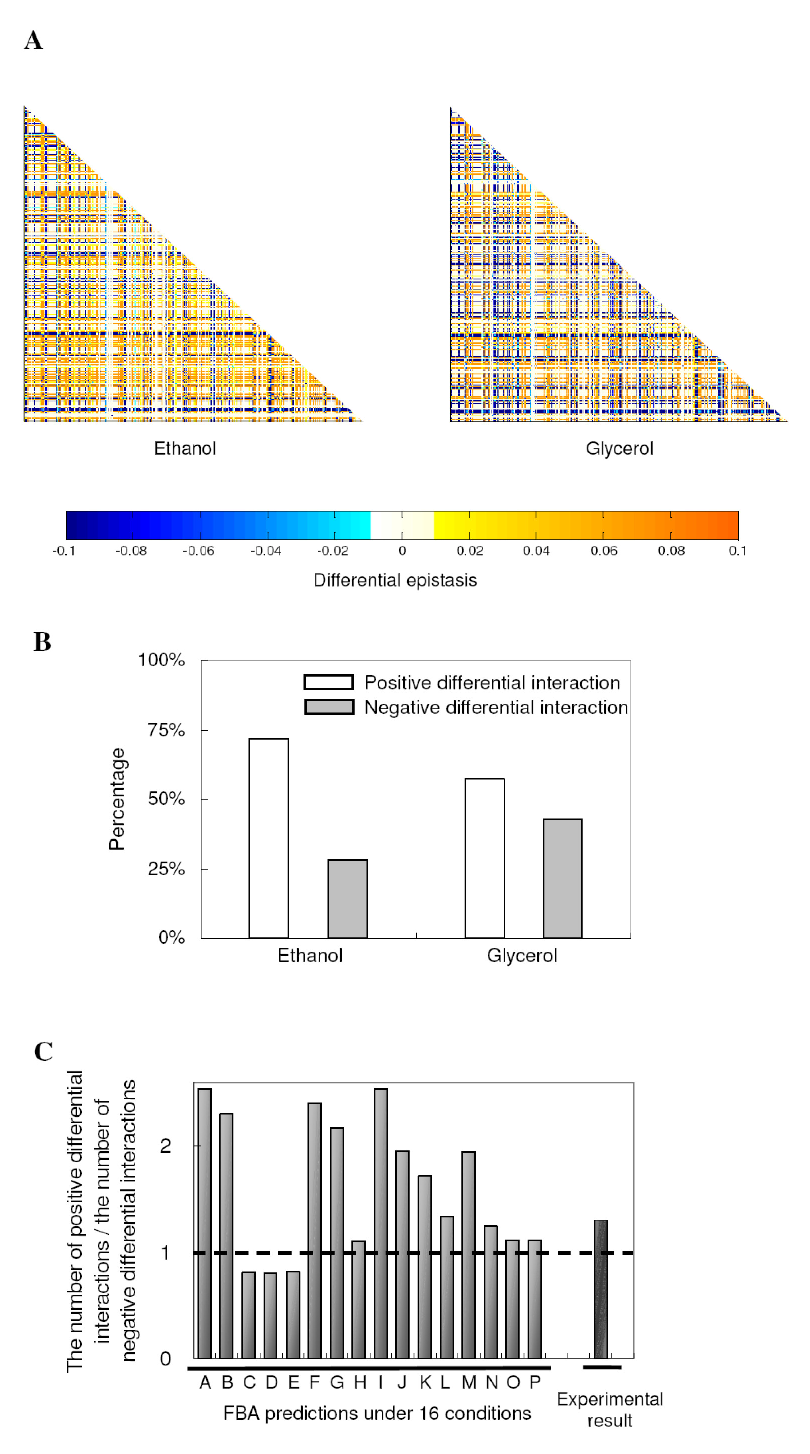
\includegraphics[height=0.95\textheight]{envFigure_1}
\end{figure}
}{}

We further investigated the sign of differential epistasis from
abundant-glucose to nutrient-limiting conditions. As shown in Figure
1A, we observed more yellow dots (positive differential epistasis)
than blue dots (negative differential epistasis) in both
panels. Indeed, as quantified in Figure 1B, 72\% and 57\% of
differential epistases are positive in ethanol and glycerol
conditions, respectively. We further explored all 16 nutrient-limiting
conditions and the results are shown in Figure 1C. In most of our
simulated conditions (13/16), there are significantly more positive
differential epistases than negative differential epistases (Binomial
test, P $<$ 10-5 for each of the 13 conditions), indicating that
epistasis tends to become more positive in nutrient-limiting
conditions. This conclusion does not depend on the criteria we used to
define differential epistasis (Figure S1).

A recent high-throughput experiment measured epistatic relations
between $\approx$~80,000 gene pairs with and without perturbation by a
DNA-damaging agent (methyl methanesulfonate, MMS). The study
represents the most comprehensive experimental study so far to explore
epistatic dynamics from a rich medium to a harsh condition
\citep{Bandyopadhyay2011}. Interestingly, the authors also found more
positive differential
epistases than negative differential epistases, which is consistent
with our general observation (Figure 1C). We further allowed maximum
growth in each condition and the general trends in our results
remained similar (Figure S2).

We found that differential epistasis had functional importance after
performing both Gene Ontology (GO) and Kyoto Encyclopedia of Genes and
Genomes (KEGG) enrichment analyses to compare genes with positive and
negative differential epistases through the glucose-abundant to
ethanol transition. We chose the ethanol condition as an example
because it is one of the most widely used conditions for the baker’s
yeast. Interestingly, we observed that 38 GO terms and 8 KEGG pathways
are enriched for positive differential epistasis, while 18 GO terms
and 1 KEGG pathways are enriched for negative differential epistasis
(Table S3). More importantly, we found positive and negative
differential epistases uniquely contribute to different aspects of
ethanol and energy metabolism. For example, positive differential
epistasis is enriched in monohydric alcohol metabolic processes,
oxidoreductase activity acting on aldehyde group donors, the TCA
cycle, and pyruvate metabolism, while negative differential epistasis
is enriched in ethanol metabolic processes and various amino acid
terms and pathways, indicating the functional importance of
differential epistasis (Table S3). This is consistent with
experimental results that show differential epistatic interactions,
rather than static epistatic interactions, are functionally related to
the response of interest \citep{Bandyopadhyay2011}.

Several system properties were found to correlate with the ratio of
the number of positive to negative differential epistases (Table
S4). A strong correlation exists between the number of essential genes
in a given condition and the ratio of positive to negative
differential epistasis on transition from high glucose to that
condition ($\rho = 0.9056$, P = 1.3905e-006), which was a better predictor
than the number of non-zero fluxes in the wild-type vector for that
environment ($\rho = 0.7131$, P = 0.0019). An even stronger predictor for
positive differential epistasis was the mean relative fitness of
single mutants in the new environment ($\rho = -0.9941$, P = 6.4340e-015);
this anticorrelation suggests that a propensity for a lower single
mutant fitness can cause a shift towards positive epistasis.

\subsection{Dynamic epistasis between nutrient-limiting conditions}

Figure 1 explored the epistasis dynamics from abundant-glucose media
to nutrient-limiting conditions. As biological systems in nature
constantly face changing environmental perturbations, it is
interesting to investigate the epistasis dynamics among
nutrient-limiting conditions. To achieve this aim, we first explored
the epistatic relationship between the same gene pairs in the two
environmental perturbations based on growth in ethanol and
glycerol. Figure 2A lists the number of gene pairs that have various
epistatic relationships. It is noteworthy to point out that,
consistent with previous published results there are significantly
more positive epistases between genes than negative ones in either
condition \citep{He2010}.

If two genes have the same sign of epistasis and
$\left|\epsilon\right| \geq 0.01$ in both conditions, they are defined
as having similar epistatic
relationship in these two conditions. To quantify epistatic dynamics
between ethanol and glycerol growth conditions, we defined the
percentage of gene pairs with similar epistatic relations to be the
number of gene pairs with similar epistasis relations shared in these
two conditions (overlap) divided by the number of gene pairs with
epistasis in either condition (union). Our results show that 79\% of
gene pairs have similar epistasis relations between these two
conditions. Figure 2B shows the distribution for the percentages of
gene pairs with similar epistasis relations between any 2 of 16
conditions, demonstrating a variable degree of epistatic similarity
between any two conditions.  This conclusion still holds when we used
different criteria to define epistatic relationships between genes
(Figure S3).

To understand the global distribution of all epistatic relations, we
considered 16 conditions together and calculated the fraction of
epistatic interactions existing in 1, 2, 3, \ldots, 15, and 16
conditions, respectively. As shown in Fig 3A, we found that there is a
U frequency distribution for the number of growth conditions in which
a specific epistatic interaction is observed. This means that
approximately 52\% of these interactions are either condition-specific
(24\%; termed dynamic) or predicted to exist in all conditions (28\%;
termed stable), and $\approx$~48\% is intermediate (exists in multiple but not
all 16 conditions). An analogous result was obtained previously, but
only for synthetic lethal interactions \citep{Harrison2007}. We also changed the
growth assumption and allowed maximum growth in each condition and
reanalyzed the global distribution of all epistatic relations. The U
frequency distribution for the number of growth conditions in which a
specific epistatic interaction is observed remained similar (Figure
S4). Based on the result in Figure 3A, we further calculated the ratio
of these three types of epistatic relations in each of the 16
environmental perturbations. As shown in Figure 3B, we found that in
each environment, $\approx$~40-60\% of epistatic interactions are stable ones
and that each specific environmental condition also has many private
epistases among genes.

\subsection{Different network properties for stable and dynamic epistasis}

Analysis on network properties can reveal various organization
principles (e.g. frequency of occurrence, centrality) for epistasis
networks \citep{Tong2004, Costanzo2010} and therefore provide valuable
information to further
distinguish stable and dynamic epistasis. To achieve this aim, we
compared networks formed by extremely stable and extremely dynamic
epistasis among genes and asked whether they have distinct network
properties. The degree distributions for both types of epistasis are
shown in Figure 4A. Interestingly, extremely stable epistatic
interactions form an exponential network architecture, which is
homogeneous, meaning that most nodes have a very similar number of
links (Figure 4A, left panel). In contrast, the extremely dynamic
epistatic interactions give rise to a scale-free network topology,
which is heterogeneous, meaning that the majority of nodes have few
links but a small number of hubs have a large number of links (Figure
4A, right panel).

In addition, we calculated three network parameters to compare these
two types of epistatic interactions. We found that the network formed
by extremely stable epistases has a smaller shortest path length, a
larger clustering coefficient and larger closeness than the network
formed by extremely dynamic epistases (Figure 4B). These results are
consistent with the scenario that genes with extremely stable
epistasis are directly linked to most other genes and form an
exponential network topology, while genes with extremely dynamic
epistasis form a scale-free network. Our results also show that the
network induced by intermediate epistases have intermediate values of
these parameters compared to that of extremely stable and extremely
dynamic epistasis networks (Tables S5 and S6).

\subsection{Co-evolution of genes with epistatic interaction}

Gene pairs with epistasis identified in real experiments usually show
similar evolutionary rates. To investigate whether two genes with
predicted epistasis also tend to co-evolve, we calculated the
evolutionary rate differences between two genes with epistasis from
FBA modeling (Fig 5A). Evolutionary rates
($d_\textnormal{N}$/$d_\textnormal{S}$) based on orthologous gene sets
from four yeast species of the genus Saccharomyces were downloaded
from a commonly used reference dataset \citep{Wall2005}. Simulations
based on the same number of gene pairs with FBA-predicted epistasis
were conducted to estimate the evolutionary rate differences for any
two randomly selected genes. As shown in Figure 5A, the gene pairs
with FBA-predicted epistatic interactions tend to have more similar
evolutionary rates than random expectation (P $<$ 10-4).

In Figure 4 we observed unique network properties for extremely stable
and extremely dynamic epistatic interactions. We further investigate
the co-evolution between genes with these two types of epistatic
relationships. As shown in Figure 5A, genes with extremely stable
epistasis tend to co-evolve (P $<$ 10-4), while the difference between
genes with extremely dynamic epistasis and random expectation becomes
much smaller (P = 0.06). The evolutionary rate difference between gene
pairs with extremely stable and extremely dynamic epistasis is also
significant (\textit{t}-test, P = 8e-6). This difference is not caused by
genes that are involved in extremely stable or extremely dynamic
epistasis, because these two groups of genes do not have significantly
different evolutionary rates (\textit{t}-test, P = 0.796, Figure 5B).

\section{Discussion}

\subsection{Natural selection in nutrient-limiting conditions}

Whether a genetic mutation has a fitness consequence depends on other
sites, a phenomenon called epistasis (see \citealt{Lehner2011} for a
recent review on
molecular mechanisms). Positive epistasis alleviates the total harm
when multiple deleterious mutations combine together and thus reduces
the effectiveness of natural selection in removing these deleterious
mutations, whereas negative epistasis plays the opposite role by
increasing the efficiency of purging deleterious mutations by natural
selection. Results from this study present an initial glimpse over
environment-induced epistasis dynamics at the genome scale. Using
differential epistasis from abundant-glucose to nutrient-limiting
conditions, our results show that epistasis between specific genes can
become more positive or more negative in nutrient-limiting conditions,
which is consistent with previous findings in small scale studies
\citep{Remold2001, Kishony2003, Cooper2005, Korona1999, Szafraniec2001,
Jasnos2008, Vassilieva2000, Baer2006, Yang2001, Fry2002,
AletheaD.Wang2009, Young2009}. However, we showed that, at the genome
scale, epistasis is
more positive in nutrient-limiting conditions. Interestingly, our
simulation results are consistent with a recent genome-wide study
between laboratory and harsh growth conditions
\citep{Bandyopadhyay2011}. How epistasis affects selection in harsh
conditions has been controversial \citep{Agrawal2010}. Our
results provide the genome-wide evidence arguing that selection might
be less effective in removing deleterious mutations in harsh
conditions, which could be one of the underlying reasons for a recent
observation that stimulation of a stress response can reduce mutation
penetrance in \textit{Caenorhabditis elegans} \citep{Casanueva2012}.

\subsection{Network properties and evolutionary patterns for stable
and dynamic epistasis}

Our results indicate that epistasis could be extremely stable or
dynamic among various environmental perturbations, which is consistent
with a previous FBA study investigating synthetic lethal relations
among non-essential genes \citep{Harrison2007}. The inclusion of
essential genes in our study allows for investigation on many
important metabolic
pathways that were not previously analyzed. Nevertheless, the
distribution of epistasis among multiple environments (Figure 3A)
remains largely unchanged from the previous study \citep{Harrison2007}
even when essential genes are included.

We also found that stable and dynamic epistatic relationships show
totally different network properties and evolutionary patterns, which
might provide new biological and evolutionary insights. The gene pairs
with stable epistases tend to co-evolve with each other. In addition,
from the biological pathway perspective, the smaller shortest path
length and larger closeness values in the stable epistasis network
both imply that genes with stable epistases tend to be functionally
associated with a large number of neighbors to form a condensed
functional network, different from genes in the dynamic epistasis
network that are loosely connected. Furthermore, the large clustering
coefficient in the stable epistasis network also supports the idea
that genes with stable epistasis interactions form a network core in
the whole epistasis network. Combined with observations in Figure 5,
this core module of epistasis in the metabolic network might represent
stable functional associations between genes that are essential for
important biological functions and evolutionary conserved even under
different environmental perturbations. The lack of co-evolution
pattern and scale-free network properties for the dynamic epistasis
network, however, might represent unstable functional associations
between genes, which may only be responsible for unique functions
under specific conditions.

\subsection{Implications and significance for exploring stable and
dynamic epistasis}

Our prediction about stable and dynamic epistasis could have important
functional applications. A recent study showed that the synthetic
lethal (negative epistasis) relationship between fumarate hydratase
and haem oxygenase can be employed successfully to identify an in
vitro drug target in hereditary leiomyomatosis and renal-cell cancer
(HLRCC) cells \citep{Frezza2011}. Exploring both dynamic and stable
epistasis could be useful in this context; stable epistatic
interactions may be
important for drug target detection in cancer or other pathogens,
whereas it may sometimes be necessary to exploit dynamic epistatic
relationships, possibly induced by treatment with an external
perturbation.

Furthermore, rational evolutionary design techniques such as OptKnock
\citep{Burgard2003} and OptGene \citep{Patil2005} attempt to find
which knockouts will enable a reaction of interest to be coupled with
growth (i.e. have positive
epistasis with growth-associated genes in a specific
environment). However, these techniques do not take into account
epistasis dynamics across different environments. In this study, we
have found that epistatic relations can be highly dynamic under
various environmental perturbations, which raises the possibility to
improve these techniques by considering epistasis dynamics in future
studies. Research on using compensatory perturbations to reach desired
network states is ongoing \citep{Cornelius2011}.

\subsection{Caveats and future directions} Though we show several
novel insights into how varying environments can influence epistasis,
several caveats should be addressed. First, the FBA modeling used in
this study, which was proven to have great predictive power and has
been successfully employed in addressing numerous research problems
\citep{Edwards2001, Shlomi2005, Smallbone2009a}, 
only includes metabolic genes. Second, even though FBA
offers the most comprehensive simulation method for studying
epistasis, there are many improvements that can be made in order to
capture the empirically observed set of epistatic interactions
\citep{Covert2001}. For example, integrating transcriptional
regulation and physical interactions into this framework could improve
the current methods in predicting epistasis and other evolutionary
processes \citep{Szappanos2011}. Related to
this point, FBA as used herein only considers the steady state and
does not take into account any dynamics or initial conditions, and
would necessarily miss any epistatic interactions that are due to
dynamics in the system, such as changing concentrations; dynamic FBA
(which is part of rFBA) might be a solution, but would likely require
about a minimum of two orders of magnitude increase in computation
time \citep{Covert2001, Varma1994}. Recent work
on new objective functions targeting metabolite turnover rather than
flux per se has also proven successful in recovering many epistases
that were previously not found with FBA \citep{Brochado2012}.

Third, in order to understand the impact of environmental
perturbations on epistasis, we used a reductive approach and only
considered one mutation type per gene to simulate the global epistatic
landscape in 16 environments. There are countless environments in
nature. Furthermore, different mutations in the same gene and the
interactions between genes and environment can likely have an even
more complex impact on the epistasis dynamics. While it would be ideal
to simulate a larger variety of environmental conditions for multiple
mutations of the same gene, the computational cost is a limiting
factor. Our previous study showed that different mutants of the same
gene could have very dynamic epistatic interaction partners in a
single environment \citep{Xu2012}. In this study, we chose to use one
mutation per gene as we are focusing on addressing how different
environments could affect gene epistasis dynamics. Nevertheless, in
order to see how sensitive our results were, we performed the analysis
for our core results by simulating 16 environments using different
growth assumption, where the organisms are allowed to have
unrestricted uptake of the limiting nutrient to obtain the maximum
growth in that condition. We found the major trends in our results are
largely unchanged (Figures S2 and S4; Table S1).

Keeping these issues in mind, our analysis uncovered several prominent
features of epistatic interactions under a variety of environmental
perturbations, and call on future effort to confirm these simulation
results using high-throughput experimental platforms. More
importantly, the enrichment of stable and dynamic epistasis provides a
new perspective to understand how biological systems may rewire
epistasis in nature.

\section{Methods}

Scripts for generating and analyzing the data can be found in the
source code repository located at
\url{https://github.com/bbarker/COBRAscripts/}. Scripts and
documentation specific to this paper are located in the subdirectory
\texttt{MyProjects/EnvironmentalEpistasisFBA}.

\subsection{Flux Balance Analysis}

Flux Balance Analysis attempts to tackle issues inherent in other
methods of metabolic modeling, such as the need to measure a large
number of parameters, slow speed of simulation, and dependence on
initial conditions \citep{Orth2010, Schellenberger2011a}. 
Other than needing a fairly complete
understanding of the reactions present in an organism, the only
measurements required to perform a genome-scale metabolic simulation
are those for determining biomass constitution or a gene expression
profile \citep{Shlomi2005, Mo2009}. Strictly speaking, FBA is a particular type of
constraint based modeling (CBM). Constraint based modeling frames the
stoichiometry that describe the reactions present in an organism as a
matrix equation with indeterminates (reaction fluxes) subject to
constraints \citep{Smallbone2009a, Mo2009}. The optimization problem
is described as follows:


\begin{equation}
\centering
\begin{tabular}{rl}
maximize   & $\mathbf{c}^T\mathbf{v}$                                     \\
subject to & $\mathbf{S v} = \frac{\D{\mathbf{x}}}{\D{t}} = \mathbf{0}$   \\
           & $\mathbf{v}_{lb} \preceq \mathbf{v} \preceq \mathbf{v}_{ub}$ \\
\end{tabular}
\end{equation}

$\mathbf{S}$ is a matrix, in which rows and columns correspond to
cellular metabolites and reactions in the reconstructed network
respectively. $\mathbf{v}$ is the reaction flux with upper and lower
bounds $\mathbf{v}_{ub}$ and $\mathbf{v}_{lb}$
respectively. Multiplying the stoichiometric matrix $\mathbf{S}$ by
the flux vector v equals the concentration change over time
($\frac{\D{\mathbf{x}}}{\D{t}}$). At steady state, the flux through
each reaction is given by $\mathbf{Sv} = \mathbf{0}$. Further details
on the underlying methods can be found in the literature 
\citep{Xu2012, Smallbone2009a, He2010}.

The fluxes of mutations employed in this analysis were restricted to
be 50\% of the wild-type fluxes found for growth rate maximization by
geometric FBA \citep{He2010}. To find new conditions with a specified carbon
source or other limiting nutrient that achieves 20\% of the
high-glucose growth rate, we can solve a linear program for the
minimization of the limiting nutrient uptake while requiring the
growth rate to be equal to 20\% of the abundant-glucose
growth-rate. For maximum growth rate conditions (Table S1, \Fig s S2
and \ref{fig:eefS4}), we allowed unrestricted uptake of the limiting nutrient to
obtain the maximum growth in that condition, up to the point where it
would reach the high-glucose growth rate. Mutations affecting protein
complexes and pleiotropic genes are handled by uniform restriction
across enzymes as described before \citep{Xu2012}.

\subsection{Definition of epistasis}

In each gene mutant pair, the epistasis value is calculated based on
the equation: $\epsilon = W_{xy} - W_xW_y$, in which $W_{xy}$ is the
fitness of an organism with two mutations in genes X and Y, whereas
$W_{x}$ or $W_{y}$ refers to the fitness of the organism with mutation
only at gene X or Y respectively. Each fitness listed previously is
calculated relative to the wild-type fitness. Absolute fitness values
are determined by the value of the biomass maximization objective
present in the model. Finally, a confidence threshold
($\left|\epsilon\right| \geq 0.01$) was applied to generate epistatic
interactions \citep{Xu2012, Costanzo2010, He2010}. We also conducted
analyses based on a different threshold for epistasis and the general
conclusions still hold in our analysis (Figures S1 and S3).

\subsection{Evolutionary rates and network parameters}

Evolutionary rates of \textit{S. cerevisiae} genes were downloaded
from supplementary materials of \citealt{Wall2005}, in which orthologs were
defined by four complete genomes of \textit{Saccharomyces} species
(\textit{Saccharomyces cerevisiae}, \textit{Saccharomyces paradoxus},
\textit{Saccharomyces mikatae} and \textit{Saccharomyces bayanus}) and
evolutionary rates at synonymous and nonsynonymous sites were
calculated based on a four-way yeast species alignment for
\textit{S. cerevisiae} genes by PAML. For the distributions in Figure
5A, we randomly sampled gene pairs with the same number of gene pairs
as in three epistasis networks (epistasis in all 16 conditions,
extremely stable epistasis, and extremely dynamic epistasis,
respectively), and calculated the average evolutionary rate
differences between random gene pairs in each of these three sample
sets. The simulations were repeated 10,000 times for each of the three
groups, which are color coded to correspond to the epistasis networks
of the same size.

Network parameters such as the shortest path length, clustering
coefficient and closeness were calculated using the computer software
Pajek, downloaded from:
\url{http://vlado.fmf.uni-lj.si/pub/networks/pajek}. The shortest path
length between two genes in a network reflects the overall network
interconnectedness; the smaller the average shortest path length is,
the higher chance that genes in this network could interact with the
other genes. The clustering coefficient of a network is a measurement
of the degree to which nodes in a network tend to cluster together;
the larger the average clustering coefficient is, the more closely the
genes are connected, forming modules. The closeness of a network
measures the centrality of nodes within a network; nodes that occur on
shortest paths with other nodes have higher closeness than those that
do not \citep{Barabasi2004}.

\section{Acknowledgments}

We firstly thank Tim Connallon for extremely helpful discussion
related to epistasis. Discussions from Dr. Huifeng Jiang, Dr. Chris
Myers, and Mr. Kaixiong Ye are also very much appreciated. This work
was supported by the startup fund from Cornell University, NSF
DEB-0949556 and NIH 1R01AI085286 awarded to Z.G

